
\section{Design Space of Sketchy Rendering\\for 2.5D Treemaps}
\label{sec:rendering}

\noindent 
Sketchiness as a visual variable is accomplished in our approach by sketchy rendering 
applied to the components a 2.5D treemap, imitating hand-drawn outlines and fillings. 

Different sketchy styles are implemented based on different NPR drawing concepts \cite{Schlechtweg1998}
such as pencils, colored pens, ballpoint pens, or markers (\autoref{fig:styles}).
As the degree of sketchiness can vary per block, 
we have to ensure that the sketchy rendering technique can be independently processed per block. 
In our approach, we focus on a small set of clearly distinguishable hand-drawn styles,
in particular outlines and textures (\autoref{fig:teaser}) that fulfill this constraint.

\subsection{Rendering of Sketchy Outlines}
\label{subsec:outlines}

\noindent
Sketchy outlines imitate lines that appear to be hand-drawn with a drawing tool.
The essential characteristics are 
(1) graphical inconsistency (the stroke's texture), 
(2) perturbation of spatial position (wobbling), and 
(3) overdraw (multiple strokes of varying intensity per line feature).

\vspace{\baselineskip}

\begin{wrapfigure}{l}{52pt}
	\vspace{-\baselineskip}
	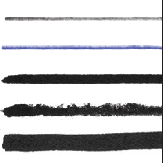
\includegraphics[width=66pt]{designspace-outline-texture}
	\vspace{-1.0\baselineskip}
\end{wrapfigure}
\noindent\textbf{Graphical Inconsistency.}
Hand-drawn strokes can vary depending on line thickness, pressure---causing a sparser
or denser texture grain and a reduced or increased color intensity respectively---as well as the type of drawing tool used.
Common drawing tools for sketching are (depicted top to bottom) graphite pencils, biros, sharpies, crayons, and markers.
The variations in grain, intensity, and thickness can be accounted for by using either image-based or procedurally-generated textures for real-time rendering.

\begin{wrapfigure}{l}{52pt}
	\vspace{-\baselineskip}
	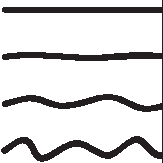
\includegraphics[width=66pt]{designspace-outline-spatial}
	\vspace{-1.0\baselineskip}
\end{wrapfigure}
\noindent\textbf{Spatial Position.}
The appearance of strokes is also determined by their straightness, 
which can be influenced  due shaking or wobbling (\emph{perturbation}) by noise. 
We use the maximum perturbation of a stroke as a control for the intensity of sketchiness \cite{Boukhelifa2012}.
For real-time rendering, 
3D spatial perturbation is implemented by subdividing  strokes (\emph{tessellation}) into multiple line segments and individually 
displacing each point by a spatially referenced offset implemented by a 3D noise texture look-up.
With the amplitude, frequency (or number of octaves), and type of noise, 
the appearance of single strokes can be further refined.
For example, white noise (high frequency) creates a highly unsettled, edgy look, 
while simplex noise causes a rather smooth and curvy appearance.
In contrast to most image-based approaches, 
our method is view-independent and produces no shower door effects. 

\begin{wrapfigure}{l}{52pt}
	\vspace{-\baselineskip}
	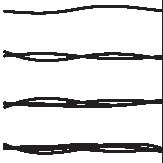
\includegraphics[width=66pt]{designspace-outline-overdraw}
	\vspace{-1.0\baselineskip}
\end{wrapfigure}
\noindent\textbf{Overdraw.}
The display of a single line is not limited to a single stroke. 
Instead, multiple strokes of the same texture but with varying perturbation can be applied (\emph{overdraw}).
We achieve this by shifting the 3D noise look-up randomly for every stroke.
Although an overdraw of strokes with varying intensities (\eg due to uneven pressure applied when drawing) allows us to increase the visualizations aesthetics, 
we do not consider it to significantly affect the perceived degree of sketchiness of outlines here.

\begin{figure*}[t!]
	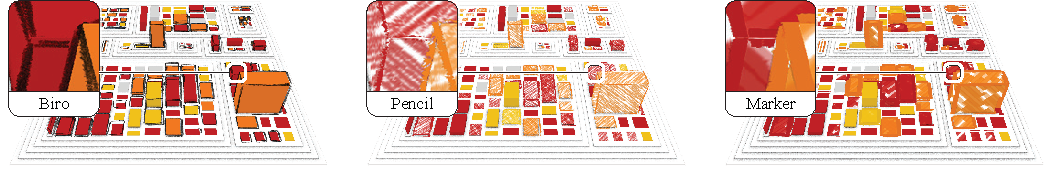
\includegraphics[width=\textwidth]{sketchiness-variations}
	\caption{Different sketchy styles: Default shading with ballpen outlines (Biro), outlines imitating colored pencils combined with slightly desaturated hatching (Pencil), thick outlines and hatches for imitating text markers (Marker).}
	\label{fig:styles}
\end{figure*}

\paragraph{Implementation.}
Sketchy outlines in 2.5D treemaps are rendered as follows: 
For all edges of all sketchy blocks an additional draw call (line draw) is dispatched.
The edges are GPU-tessellated and displaced per vertex using spatially referenced 3D offsets.
For the offsets, a single tileable, linear filtered 3D noise texture is pre-computed and scaled appropriately.
Finally, view-oriented billboards are derived along the line segments and textured via distance transformed stroke maps.
Since the number of leafs comprised by treemaps strongly varies, a level-of-detail concept as well as an appropriate effect (re)parameterization in terms of scale has not been investigated so far.

\subsection{Rendering of Sketchy Textures}
\label{subsec:surfaces}

\noindent
To render block surfaces in a sketchy style, 
we use hatch textures to modify the surface appearance such as the Pencil and Marker examples in \autoref{fig:styles}.
The design space for sketchy textures is similar to sketchy outlines; 
it includes filling style, stroke texture and stroke density.

As a replacement of solid shading in the block rendering technique, either hatching or stippling can be used.
Both convey texture, tone, and form 
by drawing closely spaced dapples or parallel as well as orthogonal strokes or stipples.
For every stroke of a texture, a homogeneous parameterization of graphical inconsistency and spatial perturbation is implied in order to maintain the blocks distinct appearance.
Varying densities of strokes might cause quite different effects---%
a cross-hatched surface displays the original color much better than a sparse hatched surface since the sparse version contains a lot more background color.
To retain the thematic mapping, hue hatching is typically used for sketchiness in information visualization \cite{Wood2012};
instead of depicting lighting and shading information, the hatching intensity indicates the degree of sketchiness (\autoref{fig:order}).

\begin{figure}[b!]
	
\includegraphics[width=\linewidth]{stylization-order-pencil}
	\caption{Sketchiness based on colored pencil drawing: a block can be rendered in a range from non-sketchy (left) to maximal sketchy (right). For it, the hatching intensity is designed to decrease evenly.}
	\label{fig:order}
\end{figure}

\paragraph{Implementation.}
For real-time rendering using hatching we use pre-rendered distance transformed Tonal Art Maps (\emph{TAMs}) \cite{Praun2001}.
A TAM is a set of texture images of different stroke densities, \ie hatching intensities, that get blended appropriately during fragment shading. 
Here, shower door effects are avoided by stroke-aware mipmapping.
In the case of strongly discretized color mapping---we prefer five buckets \cite{Boukhelifa2012}---a five-level sketchiness allows us to slightly account for shading without compromising its discernibility.
Similar to the setup for outlines, the TAMs' size and stroke-scales should be adjusted to the treemap size.

